\subsection{Can the model say when not to trust it? (RQ4)}
\label{sec:res-uncertainty}

\Cref{tab:unc} and \cref{fig:unccov} compare four ways of building 90\% prediction intervals on unseen stations.

\begin{table}[h]
\centering\small
\caption{Nominal 90\% intervals on unseen stations: empirical coverage / mean width (WQI points). ``One cat.'' is the share of visits whose whole interval lies within one category, i.e.\ the category can be stated confidently.}
\label{tab:unc}
\begin{tabular}{lcccc r}
\toprule
Subset & GPR & Split-conformal & Quantile GBM (raw) & CQR & One cat.\ (conf.) \\
\midrule
\sub{S3} & 93.1 / 10.2 & 90.3 / 9.5 & 76.9 / 7.2 & 90.9 / 9.0 & 62\% \\
\sub{S4-routine} & 91.7 / 9.6 & 91.6 / 9.1 & 74.7 / 6.6 & 91.3 / 8.5 & 63\% \\
\sub{S5} & 90.0 / 9.4 & 90.9 / 8.7 & 74.3 / 6.5 & 91.6 / 8.6 & 65\% \\
\sub{S7} & 91.1 / 3.6 & 91.4 / 3.2 & 74.1 / 4.1 & 91.7 / 5.4 & 87\% \\
\sub{I3-importance} & 89.1 / 7.3 & 90.8 / 7.0 & 77.2 / 5.3 & 91.5 / 7.5 & 72\% \\
\sub{Full-8} & 86.0 / 2.2 & 92.3 / 2.5 & 73.1 / 4.4 & 91.5 / 5.5 & 90\% \\
\bottomrule
\end{tabular}
\end{table}

\begin{figure}[t]
  \centering
  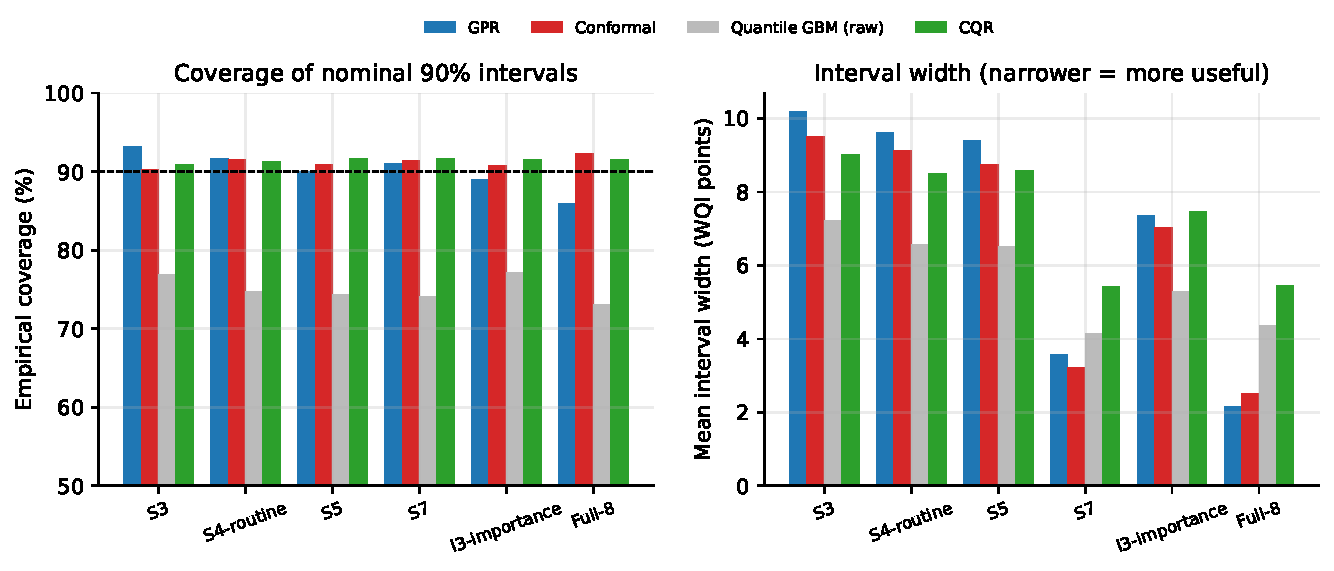
\includegraphics[width=\textwidth]{fig_unc_coverage_width.pdf}
  \caption{Coverage (left; dashed line = nominal 90\%) and mean width (right) of the four interval methods.}
  \label{fig:unccov}
\end{figure}

\paragraph{Split-conformal intervals are the method of choice.} Built around the XGBoost point prediction, with the half-width taken from inner station-grouped CV residuals, they achieve 90.3--92.3\% coverage for every subset. Their calibration curve lies on the diagonal at every level from 50\% to 95\%\optref{fig:unccal}. Their half-widths are $\pm$4.75 points for \sub{S3}, $\pm$3.5 for \sub{I3} and $\pm$1.6 for \sub{S7}. Because the guarantee is distribution-free, it does not depend on the model being correct, which is exactly the property needed at a data-scarce site. They are simple, need only one model, and are the narrowest valid intervals for the larger subsets.

\paragraph{Raw quantile regression under-covers.} Gradient-boosted 5\%/95\% quantile models reach only 73--77\% coverage at new stations, because quantiles learned on the training stations are too narrow for unseen ones. Conformalising them (CQR) restores 91--92\% coverage with intervals whose width adapts to the input. For the three- to five-parameter subsets CQR is slightly narrower than plain conformal (by 0.1--0.6 points). For \sub{S7} and \sub{Full-8}, however, it is much wider (5.4 vs.\ 3.2 and 2.5), because the quantile models are less accurate than the XGBoost point model.

\paragraph{GPR intervals are well-sized at 90\% but miscalibrated elsewhere.} For \sub{S3} the GPR curve is S-shaped\optref{fig:unccal}: 38\% coverage at nominal 50\%, but 93\% at nominal 90\%. The residuals are heavier-tailed than Gaussian. For \sub{Full-8}, GPR under-covers (86\%), because its subset-of-data fit underestimates the noise. GPR intervals are therefore usable as a rough guide but should be conformalised before reporting.

\iffull
\begin{figure}[t]
  \centering
  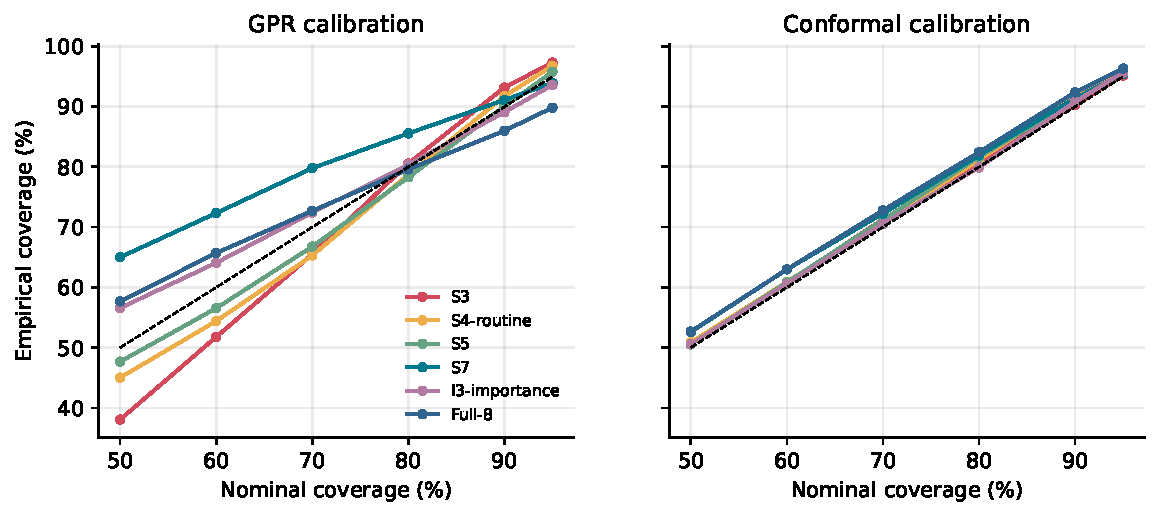
\includegraphics[width=0.85\textwidth]{fig_unc_calibration.pdf}
  \caption{Calibration of GPR (left) and split-conformal (right) intervals across nominal levels. The dashed line is perfect calibration.}
  \label{fig:unccal}
\end{figure}
\fi

\paragraph{Usefulness, not just validity.} With \sub{S3}, 62\% of unseen-station visits get an interval lying entirely inside one category. For the remaining 38\% the honest report is ``between Good and Poor'' or similar. \sub{I3} raises the share of confidently categorised visits to 72\% and \sub{S7} to 87\%. Coverage holds within every category except ``Very Poor'' under \sub{S7} (88\%). It holds both when turbidity is above its standard (93\% for \sub{S3}) and when it is below it (88\%), even though \sub{S3} cannot see turbidity. \iffull\Cref{fig:uncex} shows two unseen stations through 2020, including the monsoon minimum at the Tungabhadra (July) that the \sub{S3} model tracks.\fi

\iffull
\begin{figure}[t]
  \centering
  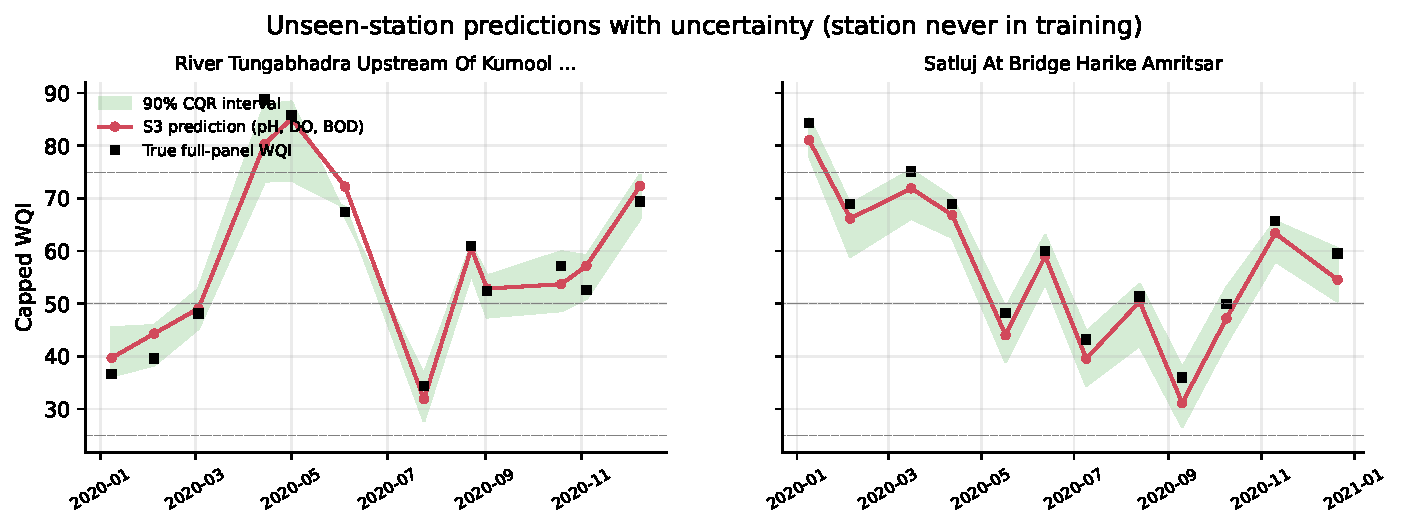
\includegraphics[width=\textwidth]{fig_unc_station_examples.pdf}
  \caption{Two stations that were never in training: true full-panel WQI (squares), \sub{S3} prediction (red) and 90\% CQR interval (green) through 2020.}
  \label{fig:uncex}
\end{figure}
\fi
